%%--------------------Chapter 3------------------------
\chapter{Thetis Design} \label{chap:thetis_design}

\section{Stakeholders} \label{sec:stakeholders}
As with any project, stakeholders are a crucial part of the design process.
Stakeholders drive certain requirements that the device must achieve in order to be accepted for operation.
On an individual level, the committee overseeing this thesis are the major stakeholders as they have a vested interest in the success or failure of the project.
However, there are some organizational-level stakeholders that have also expressed interest in the project and provided some feedback for their requirements.
A summary of the stakeholders is provided in Table \ref{tab:stakeholders}.

\begin{table}
	\caption{A summary of stakeholders of the Thetis device}
	\label{tab:stakeholders}
	\centering
	\begin{tabular}{|p{0.3\linewidth} | p{0.6\linewidth}|}
		\hline
		\rowcolor[gray]{0.8}
		\multicolumn{1}{|c|}{\textbf{Stakeholder}} & \multicolumn{1}{|c|}{\textbf{Description}} \\
		\hline
		Committee members & Individual professors who have expressed interest in the project and have agreed to assist in its development. Specifically, Dr. Wood and Dr. Weaver would like to deploy Thetis on university projects; Dr. Gutierrez has provided many requirements on the performance of the instrumentation; and Dr. Silaghi is interested in its application to autonomous navigation. \\
		\hline
		Florida Institute of \newline Technology & The university has several classes and projects where the Thetis design could be useful. The Instrumentation Design and Analysis class used Thetis as a demonstrator for designing PCBs and field experiments. Thetis was also designed with Surf Engineering Analysis in mind for students to have a new open source sensor to experiment with. \\
		\hline
		Maritime Tactical \newline Systems (MARTAC) & This corporation has expressed interest in using Thetis for research and characterizing the performance of their high speed catamarans in open-water testing \\
		\hline
		NSWC Carderock - \newline Combatant Craft Division (CCD) & This three-letter agency of the government has expressed interest in using Thetis as a testing and evaluation tool for small unmanned crafts \\
		\hline
	\end{tabular}
\end{table}

\subsection{Hands-On Users} \label{ssec:hands_on_users}

\section{Design Rationale} \label{sec:design_rationale}
Thetis is envisioned as an open-source all-in-one data logging solution for use in research projects.
The device incorporates multiple sensors, GPS tracking, and a WiFi-capable microcontroller in order to enable as many features as can be envisioned by the end users.
One of the driving considerations was the small footprint.
Thetis Revision F is designed to fit into one of the smallest IP67-rated enclosures available on the market [LINK].  
This tiny form factor allows it to be inconspicuously mounted to any floating body like surfboards, scale models, or wave buoys without upsetting their inertial characteristics or impeding nominal operation.

Further discussions with stakeholders later in the design process envisioned a new iteration, Revision G, that had a larger footprint, but added more capabilities like CANbus integration and several connection ports for different communication protocols.
This revision is meant for deployment on vessels that have a NMEA2000 communications bus.
This bus allows the device to be powered from the boat's power supply and communicate data to a central controller.
These features are extremely important for the final application where Thetis is meant to feed data into a navigation algorithm for the safe passage of unmanned vessels.

\subsection{Problem Description} \label{ssec:problem_desc}
Tracking the inertial movements of small floating bodies in-situ is difficult for small-scale or student-led experiments.
The price of the measurement instruments and the data acquisition computers (DAQs) offers a high bar for entry for these projects.
Also, the size of these instruments and DAQs can negatively impact the performance or operation of small floating bodies so they cannot be effectively used.
This forces classrooms and organizations to either neglect collecting inertial data or using bulky, unreliable prototype setups using off-the-shelf components

\subsection{Mission Statement} \label{ssec:mission_statement}
Thetis aims to democratize the inertial measurement and tracking space for small scale experiments by implementing an open-source, feature-rich, all-in-one solution to monitoring the movements of floating bodies.

\subsection{Stakeholder Requirements} \label{ssec:stakeholder_reqs}
Interviews with the stakeholders occurred over several months and informed a set of requirements that they determined were necessary for the project's success.

\begin{itemize}
	\item[\textbf{SR 01}] - The system shall be able to record acceleration, rotation rate, orientation, and position
	\item[\textbf{SR 02}] - The system shall be able to fit into a small IP67-rated, or better, enclosure
	\item[\textbf{SR 03}] - The system shall be able to fit into a small IP67-rated, or better, enclosure
	\item[\textbf{SR 04}] - The system shall be cheaper than \$200 per unit
	\item[\textbf{SR 05}] - The system shall use components that are readily available COTS
	\item[\textbf{SR 06}] - The system designs shall be open source for modification by students
	\item[\textbf{SR 07}] - The system shall communicate intra-device using known IEEE standards (e.g. SPI/I2C/UART/etc)
	\item[\textbf{SR 08}] - The system shall communicate extra-device using WiFi and USB
	\item[\textbf{SR 09}] - They system shall have enough on-board storage for 4 hours of continuously logging at 64 Hz
	\item[\textbf{SR 10}] - Thetis Revision G shall be able to communicate extra-device using CANbus
	\item[\textbf{SR 11}] - The system shall have redundant storage for device and communication events
\end{itemize}


\subsection{Risk Identification} \label{ssec:risk_identification}
The following tables explore some of the larger risks associated with each of the stakeholder requirements.
Risks are categorized into several types: Technical, Cost, Schedule, Organizational, and Operational.
Each risk has an associated consequence on the project's development and a severity rating from "Low" to "High".
With every risk, we can apply a mitigation to it to reduce the severity of the consequence.

\paragraph*{Technical Risks} These are risks that pose a technical challenge to the project such as sensor accuracies, programming difficulty, or component specifications. 
These risks are likely to impede the development of Thetis by showing up during testing and forcing workarounds after the fact, rather than before.

\paragraph*{Cost Risks} These risks pose a threat to Thetis's development budget.
They are more likely to manifest in the supply chain of Thetis, especially in the after effects of the COVID-19 pandemic and the chaos of the chip shortage.
More often, mitigating these risks requires some careful planning and a larger budget and will typically not impede the development process.

\paragraph*{Schedule Risks} By delaying the program's development, Schedule Risks are the most notorious and costly of them all.
These risks manifest as delays in development or the supply chain and can significantly impact the expected delivery time of the device.
They also are prominent across all phases of the design process from planning to testing and are only mitigated, but never eliminated during the design spiral.

\paragraph*{Organization Risks} The stakeholders represent various organizations that have an interest in Thetis.
This risk type poses a problem for the specific stakeholder organization and their interests.
This can be viewed from the political, economical, or schedule points of view as these are important considerations for the stakeholders.

\paragraph*{Operational Risks} These risks challenge end users of the device while they are testing.
Most of them can be mitigated in the design process by working directly with the end users and ensuring their concerns are met.
However, the majority of them will only manifest during testing and must be mitigated after the fact.
This could mean substantial cost increases and schedule delays depending on the severity of the risk.

\begin{landscape}


% ==================================
% === STAKEHOLDER REQUIREMENT XX ===
% ==================================


% \paragraph*{SR XX} - 

% {\fontsize{8pt}{8pt}\selectfont
% \begin{longtable}{| p{0.12\linewidth} | p{0.16\linewidth} |  p{0.20\linewidth} | p{0.08\linewidth} | p{0.20\linewidth} | p{0.08\linewidth} |}
% 	\hline \endlastfoot
	
% 	\hline
% 	\rowcolor[gray]{0.8}
% 	\multicolumn{6}{|c|}{ } \\
% 	\hline
% 	\textbf{Stakeholder:} & \multicolumn{5}{|l|}{} \\
% 	\hline
% 	\textbf{Rationale:} & \multicolumn{5}{|p{0.8\linewidth}|}{} \\
% 	\hline
% 	\textbf{Fit Criterion:} & \multicolumn{5}{|p{0.8\linewidth}|}{} \\
% 	\hline
% 	\rowcolor[gray]{0.8}
% 	\multicolumn{6}{|c|}{ } \\
% 	\hline
% 	\textbf{Risk} & \textbf{Risk Issue} & \textbf{Risk Consequence} & \textbf{Initial Risk} & \textbf{Risk Mitigation} & \textbf{Risk \newline After \newline Mitigation} \\
% 	\hline
% 	Technical \newline Assessment &  &  & \cellcolor{} &  & \cellcolor{} \\
% 	\hline
% 	Cost \newline Assessment &  &  & \cellcolor{} &  & \cellcolor{} \\
% 	\hline
% 	Schedule \newline Assessment &  &  & \cellcolor{} &  & \cellcolor{} \\
% 	\hline
% 	Organizational \newline Assessment &  &  & \cellcolor{}  &  & \cellcolor{}  \\
% 	\hline
% 	Operational \newline Assessment &  &  & \cellcolor{} &  & \cellcolor{}
% 	\label{tab:sr01_feasibility}
% \end{longtable}
% }
% \newpage


% ==================================
% === STAKEHOLDER REQUIREMENT 01 ===
% ==================================


\paragraph*{SR 01} - The system shall be able to record acceleration, rotation rate, orientation, and position

{\fontsize{8pt}{8pt}\selectfont
\begin{longtable}{| p{0.12\linewidth} | p{0.16\linewidth} |  p{0.20\linewidth} | p{0.08\linewidth} | p{0.20\linewidth} | p{0.08\linewidth} |}
	\hline \endlastfoot
	
	\hline
	\rowcolor[gray]{0.8}
	\multicolumn{6}{|c|}{ } \\
	\hline
	\textbf{Stakeholder:} & \multicolumn{5}{|l|}{Dr. Stephen Wood} \\
	\hline
	\textbf{Rationale:} & \multicolumn{5}{|p{0.8\linewidth}|}{The system needs to be able to record the inertial characteristics of a floating body} \\
	\hline
	\textbf{Fit Criterion:} & \multicolumn{5}{|p{0.8\linewidth}|}{This will be accomplished using a 9-DOF IMU and GPS receiver with accuracies not to exceed one standard deviation of a reference source} \\
	\hline
	\rowcolor[gray]{0.8}
	\multicolumn{6}{|c|}{ } \\
	\hline
	\textbf{Risk} & \textbf{Risk Issue} & \textbf{Risk Consequence} & \textbf{Initial Risk} & \textbf{Risk Mitigation} & \textbf{Risk \newline After \newline Mitigation} \\
	\hline
	Technical \newline Assessment & The IMU and/or GPS will report measurements that have a high margin of error and little consistency & Worthless data for analysis & \cellcolor{yellow} Medium & Selection of sensors that have decent accuracy and low drift. \newline Use a \emph{tuned} Kalman filter to improve reported sensor accuracy & \cellcolor{green} Low \\
	\hline
	Cost \newline Assessment & Chip shortage as a result of the COVID-19 pandemic. & Unable to find appropriate components. \newline Any found components are prohibitively expensive & \cellcolor{yellow} Medium & Find components that are in stock and order in bulk. & \cellcolor{yellow} Medium \\
	\hline
	Schedule \newline Assessment & Sensor fusion algorithms are difficult to implement and tune. & Schedule overrun trying to tune the algorithms. \newline Inaccuracies introduced through improper tuning. & \cellcolor{yellow} Medium & Good programming practices to make tuning easier during testing. & \cellcolor{green} Low \\
	\hline
	Organizational \newline Assessment & Lack of subject matter experts & Project cost and schedule delays & \cellcolor{green} Low & In-house team available. \newline Can reduce scope, as needed. \newline Proper documentation of progress and scheduled design reviews and consultations & \cellcolor{green} Low \\
	\hline
	Operational \newline Assessment & Unreliable sensors. & Device fails and does not recover during testing; lost data & \cellcolor{yellow} Medium & Reliability analysis and testing required. & \cellcolor{green} Low
	\label{tab:sr01_feasibility}
\end{longtable}
}
\newpage


% ==================================
% === STAKEHOLDER REQUIREMENT 02 ===
% ==================================


\paragraph*{SR 02} - The system shall be able to fit into a small IP67-rated, or better, enclosure

{\fontsize{8pt}{8pt}\selectfont
\begin{longtable}{| p{0.12\linewidth} | p{0.16\linewidth} |  p{0.20\linewidth} | p{0.08\linewidth} | p{0.20\linewidth} | p{0.08\linewidth} |}
	\hline \endlastfoot
	
	\hline
	\rowcolor[gray]{0.8}
	\multicolumn{6}{|c|}{ } \\
	\hline
	\textbf{Stakeholder:} & \multicolumn{5}{|l|}{Dr. Robert Weaver} \\
	\hline
	\textbf{Rationale:} & \multicolumn{5}{|p{0.8\linewidth}|}{Thetis's electronics need to be independently sealed from the elements, including being temporarily submerged } \\
	\hline
	\textbf{Fit Criterion:} & \multicolumn{5}{|p{0.8\linewidth}|}{The selected enclosure should have a UL-listing and have a verified IP rating that fits the requirement.} \\
	\hline
	\rowcolor[gray]{0.8}
	\multicolumn{6}{|c|}{ } \\
	\hline
	\textbf{Risk} & \textbf{Risk Issue} & \textbf{Risk Consequence} & \textbf{Initial Risk} & \textbf{Risk Mitigation} & \textbf{Risk \newline After \newline Mitigation} \\
	\hline
	Technical \newline Assessment & Unable to find a small enough IP-rated enclosure & Need to increase size that may violate size restrictions & \cellcolor{yellow} Medium & Extensive searching of online retailers of catalogs & \cellcolor{green} Low \\
	\hline
	Cost \newline Assessment & Small IP-67 rated enclosures are a niche item that may have to be custom-ordered and therefore expensive. & Enclosures may be prohibitively expensive and drive up program costs & \cellcolor{green} Low & Find reputable suppliers and order enclosures in bulk, if possible. & \cellcolor{green} Low \\
	\hline
	Schedule \newline Assessment & If the enclosures have to be custom ordered, there may be an extended lead time for delivery & Schedule orverruns & \cellcolor{yellow} Medium & Find reputable suppliers and order in bulk well ahead of time. \newline maintain a stock of several enclosures as spares. & \cellcolor{green} Low \\
	\hline
	Organizational \newline Assessment & N/A & N/A & \cellcolor[gray]{0.8} & N/A & \cellcolor[gray]{0.8} \\
	\hline
	Operational \newline Assessment & IP-rating is not valid. \newline Enclosure is not fully sealed. \newline Operation exceeds rated limits & Chamber floods, damaging equipment, causing a potential fire hazard and data loss. & \cellcolor{red} High & Reputable supplier and traceable IP-rating. \newline End user vigilence to ensure enclosure is fully closed and sealed. & \cellcolor{yellow} Medium
	\label{tab:sr02_feasibility}
\end{longtable}
}
\newpage

% ==================================
% === STAKEHOLDER REQUIREMENT 03 ===
% ==================================


\paragraph*{SR 03} - The system shall be able to be powered by battery for more than 4 hours continuously

{\fontsize{8pt}{8pt}\selectfont
\begin{longtable}{| p{0.12\linewidth} | p{0.16\linewidth} |  p{0.20\linewidth} | p{0.08\linewidth} | p{0.20\linewidth} | p{0.08\linewidth} |}
	\hline \endlastfoot
	
	\hline
	\rowcolor[gray]{0.8}
	\multicolumn{6}{|c|}{ } \\
	\hline
	\textbf{Stakeholder:} & \multicolumn{5}{|l|}{Dr. Robert Weaver} \\
	\hline
	\textbf{Rationale:} & \multicolumn{5}{|p{0.8\linewidth}|}{Thetis is expected to deploy for a minimum of 3 hours on a typical deployment. Need margin for battery chemistry and preparation time.} \\
	\hline
	\textbf{Fit Criterion:} & \multicolumn{5}{|p{0.8\linewidth}|}{The device shall be deployed for a long period and } \\
	\hline
	\rowcolor[gray]{0.8}
	\multicolumn{6}{|c|}{ } \\
	\hline
	\textbf{Risk} & \textbf{Risk Issue} & \textbf{Risk Consequence} & \textbf{Initial Risk} & \textbf{Risk Mitigation} & \textbf{Risk \newline After \newline Mitigation} \\
	\hline
	Technical \newline Assessment & Device is not turned off before battery voltage is critically low & Battery is damaged and needs to be replaced; fire hazard & \cellcolor{yellow} Medium & Build the power regulator such that the device auto turns off before battery is damaged & \cellcolor{green} Low \\
	\hline
	Cost \newline Assessment & Larger capacity batteries are more expensive. \newline Damaged batteries need to be replaced & Cost overruns & \cellcolor{green} Low & Order batteries in bulk and ensure spares are available & \cellcolor{green} Low \\
	\hline
	Schedule \newline Assessment & If there are no spares, there may be delays in testing schedule & Any critical testing may have to be delayed, resulting in program delays & \cellcolor{green} Low & Order batteries in bulk and ensure spares are available & \cellcolor{green} Low \\
	\hline
	Organizational \newline Assessment & N/A & N/A & \cellcolor[gray]{0.8} & N/A & \cellcolor[gray]{0.8} \\
	\hline
	Operational \newline Assessment & Battery does not have enough capacity to support a 4 hour deployment & Data is lost & \cellcolor{yellow} Medium & Conservative power analysis and choosing an oversized battery. & \cellcolor{green} Low
	\label{tab:sr03_feasibility}
\end{longtable}
}
\newpage

% ==================================
% === STAKEHOLDER REQUIREMENT 04 ===
% ==================================


\paragraph*{SR 04} - The system shall be cheaper than \$200 per unit

{\fontsize{8pt}{8pt}\selectfont
\begin{longtable}{| p{0.12\linewidth} | p{0.16\linewidth} |  p{0.20\linewidth} | p{0.08\linewidth} | p{0.20\linewidth} | p{0.08\linewidth} |}
	\hline \endlastfoot

	\hline
	\rowcolor[gray]{0.8}
	\multicolumn{6}{|c|}{ } \\
	\hline
	\textbf{Stakeholder:} & \multicolumn{5}{|l|}{Dr. Robert Weaver} \\
	\hline
	\textbf{Rationale:} & \multicolumn{5}{|p{0.8\linewidth}|}{Thetis is designed to be a cheap, expendable unit so that, when damaged by students, it is financially feasible to replace it. It needs to be cheaper than comparable devices} \\
	\hline
	\textbf{Fit Criterion:} & \multicolumn{5}{|p{0.8\linewidth}|}{The Bill of Materials for Thetis shall not exceed the required threshold.} \\
	\hline
	\rowcolor[gray]{0.8}
	\multicolumn{6}{|c|}{ } \\
	\hline
	\textbf{Risk} & \textbf{Risk Issue} & \textbf{Risk Consequence} & \textbf{Initial Risk} & \textbf{Risk Mitigation} & \textbf{Risk \newline After \newline Mitigation} \\
	\hline
	Technical \newline Assessment & Cheaper components (sensors) that are not as precise or accurate. & Less accurate data that may not be useful for analysis & \cellcolor{yellow} Medium & Use a \emph{tuned} Kalman filter to improve reported sensor accuracy & \cellcolor{green} Low \\
	\hline
	Cost \newline Assessment & Chip shortage as a result of the COVID-19 pandemic. \newline Small IP-67 rated enclosures are a niche item that may have to be custom-ordered & Parts significantly inflate the Bill of Materials cost & \cellcolor{yellow} Meidum & Source from reputable suppliers and purchase in bulk & \cellcolor{yellow} Medium \\
	\hline
	Schedule \newline Assessment & N/A & N/A & \cellcolor[gray]{0.8} & N/A & \cellcolor[gray]{0.8} \\
	\hline
	Organizational \newline Assessment & Bill of Materials cost exceeds requirement limit. \newline Development costs become too expensive & Invested stakeholders may pull support. \newline Hardware development slows or stops & \cellcolor{red} High & Purchase materials in bulk, when possible. \newline Use proper development techniques and analysis to reduce the number of hardware iterations and cost  & \cellcolor{yellow} Medium \\
	\hline
	Operational \newline Assessment & Cheaper, not as reliable parts. & Unexpected and unrecoverable failures during deployments & \cellcolor{yellow} Medium & Reliability analysis and testing required. & \cellcolor{green} Low
	\label{tab:sr04_feasibility}
\end{longtable}
}
\newpage


% ==================================
% === STAKEHOLDER REQUIREMENT 05 ===
% ==================================


\paragraph*{SR 05} - The system shall use components that are readily available COTS

{\fontsize{8pt}{8pt}\selectfont
\begin{longtable}{| p{0.12\linewidth} | p{0.16\linewidth} |  p{0.20\linewidth} | p{0.08\linewidth} | p{0.20\linewidth} | p{0.08\linewidth} |}
	\hline \endlastfoot
	
	\hline
	\rowcolor[gray]{0.8}
	\multicolumn{6}{|c|}{ } \\
	\hline
	\textbf{Stakeholder:} & \multicolumn{5}{|l|}{Dr. Stephen Wood} \\
	\hline
	\textbf{Rationale:} & \multicolumn{5}{|p{0.8\linewidth}|}{Using commercial off the shelf parts will reduce development time and costs. COTS parts will also make repair and maintenance easier} \\
	\hline
	\textbf{Fit Criterion:} & \multicolumn{5}{|p{0.8\linewidth}|}{All parts used on Thetis must be available from commercial suppliers and catalogs.} \\
	\hline
	\rowcolor[gray]{0.8}
	\multicolumn{6}{|c|}{ } \\
	\hline
	\textbf{Risk} & \textbf{Risk Issue} & \textbf{Risk Consequence} & \textbf{Initial Risk} & \textbf{Risk Mitigation} & \textbf{Risk \newline After \newline Mitigation} \\
	\hline
	Technical \newline Assessment & N/A & N/A & \cellcolor[gray]{0.8} & N/A & \cellcolor[gray]{0.8} \\
	\hline
	Cost \newline Assessment & Chip shortage as a result of the COVID-19 pandemic. \newline Small IP-67 rated enclosures are a niche item that may have to be custom-ordered & Parts significantly inflate the Bill of Materials cost & \cellcolor{yellow} Medium & Source from reputable suppliers and purchase in bulk & \cellcolor{green} Low \\
	\hline
	Schedule \newline Assessment & Parts are not available. \newline Small enclosure may have a long lead time & Development schedule should be delayed & \cellcolor{yellow} Medium & Order parts in bulk and ensure spares are available & \cellcolor{green} Low \\
	\hline
	Organizational \newline Assessment & The small enclosure may no longer be available from a commercial supplier & Forces a new design iteration to fit a new enclosure. \newline Forces end users to adapt to a new enclosure & \cellcolor{green} Low & Work with supplier to ensure supply chain; order in bulk. \newline 3D print older enclosure, if COTS is no longer available & \cellcolor{green} Low \\
	\hline
	Operational \newline Assessment & N/A & N/A & \cellcolor[gray]{0.8} & N/A & \cellcolor[gray]{0.8}
	\label{tab:sr05_feasibility}
\end{longtable}
}
\newpage


% ==================================
% === STAKEHOLDER REQUIREMENT 06 ===
% ==================================


\paragraph*{SR 06} - The system designs shall be open source for modification by students

{\fontsize{8pt}{8pt}\selectfont
\begin{longtable}{| p{0.12\linewidth} | p{0.16\linewidth} |  p{0.20\linewidth} | p{0.08\linewidth} | p{0.20\linewidth} | p{0.08\linewidth} |}
	\hline \endlastfoot
	
	\hline
	\rowcolor[gray]{0.8}
	\multicolumn{6}{|c|}{ } \\
	\hline
	\textbf{Stakeholder:} & \multicolumn{5}{|l|}{Dr. Robert Weaver} \\
	\hline
	\textbf{Rationale:} & \multicolumn{5}{|p{0.8\linewidth}|}{Thetis will need to be maintained while students use it for class projects. Therefore, they will need to have the ability to directly modify the hardware and software.} \\
	\hline
	\textbf{Fit Criterion:} & \multicolumn{5}{|p{0.8\linewidth}|}{All of the code and hardware will be published open source in GitHub repositories under an MIT license.} \\
	\hline
	\rowcolor[gray]{0.8}
	\multicolumn{6}{|c|}{ } \\
	\hline
	\textbf{Risk} & \textbf{Risk Issue} & \textbf{Risk Consequence} & \textbf{Initial Risk} & \textbf{Risk Mitigation} & \textbf{Risk \newline After \newline Mitigation} \\
	\hline
	Technical \newline Assessment & Designs are modified by students who unknowingly break functionality & Disabling or "bricking" Thetis, making it useless. \newline Loss of development history/"good" designs & \cellcolor{green} Low & GitHub tracks all commits and history. \newline "Good" designs are published as release snapshots and cannot be lost. & \cellcolor{green} Low \\
	\hline
	Cost \newline Assessment & New design modifications require more investment & Program cost increases as students change the design & \cellcolor{green} Low & Ensure that any design modifications go through a design review and adds substantial value to Thetis & \cellcolor{green} Low \\
	\hline
	Schedule \newline Assessment & New designs may require additional development time & New additions may not be ready in time for when students need them & \cellcolor{green} Low & Ensure a ready supply of spare parts. \newline Proper design practices to ensure students can easily add features & \cellcolor{green} Low \\
	\hline
	Organizational \newline Assessment & Thetis design may not be patentable and commercialized & Thetis cannot be patented since it is published open source & \cellcolor{red} High & Thetis can still be commercialized by providing board assembly and support services & \cellcolor{green} Low \\
	\hline
	Operational \newline Assessment & Vulnerabilities are found and exploited by bad actors & User data can be compromised \newline WiFi capability opens an attack vector to local network & \cellcolor{green} Low & Avoid implementation of OTA software updates \newline Use proper security techniques for FTP username and password & \cellcolor{green} Low
	\label{tab:sr06_feasibility}
\end{longtable}
}
\newpage

% ==================================
% === STAKEHOLDER REQUIREMENT 07 ===
% ==================================


\paragraph*{SR 07} - The system shall communicate intra-device using known IEEE standards (e.g. SPI/I2C/UART/etc) 

{\fontsize{8pt}{8pt}\selectfont
\begin{longtable}{| p{0.12\linewidth} | p{0.16\linewidth} |  p{0.20\linewidth} | p{0.08\linewidth} | p{0.20\linewidth} | p{0.08\linewidth} |}
	\hline \endlastfoot
	
	\hline
	\rowcolor[gray]{0.8}
	\multicolumn{6}{|c|}{ } \\
	\hline
	\textbf{Stakeholder:} & \multicolumn{5}{|l|}{Dr. Hector Gutierrez} \\
	\hline
	\textbf{Rationale:} & \multicolumn{5}{|p{0.8\linewidth}|}{Using standard communication busses to send to data between ICs on the device makes development and integration easier.} \\
	\hline
	\textbf{Fit Criterion:} & \multicolumn{5}{|p{0.8\linewidth}|}{} \\
	\hline
	\rowcolor[gray]{0.8}
	\multicolumn{6}{|c|}{ } \\
	\hline
	\textbf{Risk} & \textbf{Risk Issue} & \textbf{Risk Consequence} & \textbf{Initial Risk} & \textbf{Risk Mitigation} & \textbf{Risk \newline After \newline Mitigation} \\
	\hline
	Technical \newline Assessment & Selected ICs do not use a standard communication bus to transfer data to a microcontroller & Development time will need to be spent on a custom protocol layer & \cellcolor{yellow} Medium & Read device datasheets carefully to ensure they use standard protocols & \cellcolor{green} Low \\
	\hline
	Cost \newline Assessment & N/A & N/A & \cellcolor[gray]{0.8} & N/A & \cellcolor[gray]{0.8} \\
	\hline
	Schedule \newline Assessment & Selected ICs do not use a standard communication bus to transfer data to a microcontroller & Development time will need to be spent on a custom protocol layer & \cellcolor{yellow} Medium & Read device datasheets carefully to ensure they use standard protocols & \cellcolor{green} Low \\
	\hline
	Organizational \newline Assessment & Selected ICs do not use a standard communication bus to transfer data to a microcontroller & Future developers will have to study the custom protocol layer in order to understand how to add features & \cellcolor{yellow} Medium & Read device datasheets carefully to ensure they use standard protocols & \cellcolor{green} Low \\
	\hline
	Operational \newline Assessment & Selected ICs do not use a standard communication bus to transfer data to a microcontroller & Unintended bugs or data mistakes may be introduced by using a custom protocol layer & \cellcolor{yellow} Medium & Read device datasheets carefully to ensure they use standard protocols & \cellcolor{green} Low
	\label{tab:sr07_feasibility}
\end{longtable}
}
\newpage


% ==================================
% === STAKEHOLDER REQUIREMENT 08 ===
% ==================================


\paragraph*{SR 08} - The system shall communicate extra-device using WiFi and USB 

{\fontsize{8pt}{8pt}\selectfont
\begin{longtable}{| p{0.12\linewidth} | p{0.16\linewidth} |  p{0.20\linewidth} | p{0.08\linewidth} | p{0.20\linewidth} | p{0.08\linewidth} |}
	\hline \endlastfoot
	
	\hline
	\rowcolor[gray]{0.8}
	\multicolumn{6}{|c|}{ } \\
	\hline
	\textbf{Stakeholder:} & \multicolumn{5}{|l|}{Dr. Robert Weaver} \\
	\hline
	\textbf{Rationale:} & \multicolumn{5}{|p{0.8\linewidth}|}{A physical USB connection is crucial for programming and debugging Thetis. A WiFi connection would allow for wireless programming and data off-loading} \\
	\hline
	\textbf{Fit Criterion:} & \multicolumn{5}{|p{0.8\linewidth}|}{The microcontroller shall have a USB-compatible PHY and WiFi capability.} \\
	\hline
	\rowcolor[gray]{0.8}
	\multicolumn{6}{|c|}{ } \\
	\hline
	\textbf{Risk} & \textbf{Risk Issue} & \textbf{Risk Consequence} & \textbf{Initial Risk} & \textbf{Risk Mitigation} & \textbf{Risk \newline After \newline Mitigation} \\
	\hline
	Technical \newline Assessment & WiFi performance (speed/range) is too low and unacceptable & Data offloading is cumbersome. \newline Unable to monitor device while deployed & \cellcolor{yellow} Medium & Select microcontroller with known good WiFi-performance. \newline Select an appropriate antenna for the situation & \cellcolor{green} Low \\
	\hline
	Cost \newline Assessment & WiFi is not useful and not fully utilized & Cost per microcontroller is needlessly increased; inflated bill of materials cost & \cellcolor{yellow} Medium & Verify that WiFi functionality is desired by Stakeholders and end-users & \cellcolor{green} Low \\
	\hline
	Schedule \newline Assessment & Implementing WiFi functionality is difficult and increases complexity; feature creep. & Increased time to develop front end interface; schedule overruns & \cellcolor{red} High & Agile management to limit feature creep & \cellcolor{yellow} Medium \\
	\hline
	Organizational \newline Assessment & Some stakeholders may have electromagnetic emissions restrictions & To comply, WiFi functionality will need to be able to be disabled & \cellcolor{green} Low & Allow WiFi features to be disabled by uploading new firmware without those features, or allow users to toggle this function on/off in runtime using a configuration file. & \cellcolor{green} Low \\
	\hline
	Operational \newline Assessment & Operators may not have device that can connect to the device over WiFi & Data cannot be offloaded easily in-situ. \newline Wireless monitoring not possible & \cellcolor{green} Low & Ensure that there is always a physical backup for offloading data. \newline Physical lights or other indictors to display system status & \cellcolor{green} Low
	\label{tab:sr08_feasibility}
\end{longtable}
}
\newpage


% ==================================
% === STAKEHOLDER REQUIREMENT 09 ===
% ==================================


\paragraph*{SR 09} - They system shall have enough on-board storage for 4 hours of continuously logging at 64 Hz

{\fontsize{8pt}{8pt}\selectfont
\begin{longtable}{| p{0.12\linewidth} | p{0.16\linewidth} |  p{0.20\linewidth} | p{0.08\linewidth} | p{0.20\linewidth} | p{0.08\linewidth} |}
	\hline \endlastfoot
	
	\hline
	\rowcolor[gray]{0.8}
	\multicolumn{6}{|c|}{ } \\
	\hline
	\textbf{Stakeholder:} & \multicolumn{5}{|l|}{Dr. Robert Weaver} \\
	\hline
	\textbf{Rationale:} & \multicolumn{5}{|p{0.8\linewidth}|}{Thetis will be deployed for several hours and needs to continuously record data. Data rate should be as fast as possible to capture higher frequency oscillations.} \\
	\hline
	\textbf{Fit Criterion:} & \multicolumn{5}{|p{0.8\linewidth}|}{Storage devices shall be large enough to support a full-length deployment and record all data as fast as possible (>64 Hz)} \\
	\hline
	\rowcolor[gray]{0.8}
	\multicolumn{6}{|c|}{ } \\
	\hline
	\textbf{Risk} & \textbf{Risk Issue} & \textbf{Risk Consequence} & \textbf{Initial Risk} & \textbf{Risk Mitigation} & \textbf{Risk \newline After \newline Mitigation} \\
	\hline
	Technical \newline Assessment & Logger is not able to consistently achieve 64 Hz rate & Significant data loss on higher frequency oscillations & \cellcolor{yellow} Medium & Utilize fast storage mediums. \newline Increase microcontroller and communication clock speeds & \cellcolor{green} Low \\
	\hline
	Cost \newline Assessment & Small flash chips will not be sufficient to store the amount of data & More expensive data storage devices (micro SD cards) will have to be used; increase bill of materials cost & \cellcolor{yellow} & Find cheapest storage devices that can be used & \cellcolor{green} Low \\
	\hline
	Schedule \newline Assessment & Optimizing the logging functionality will take significant development time to be consistently as fast as possible & Schedule overruns & \cellcolor{red} High & Proper programming practices to optimize code wherever possible; reduce refactors & \cellcolor{yellow} Medium \\
	\hline
	Organizational \newline Assessment & N/A & N/A & \cellcolor[gray]{0.8}  & N/A & \cellcolor[gray]{0.8}  \\
	\hline
	Operational \newline Assessment & Inertial movements and oscillations will occur at higher frequencies than can be reasonably measured (>16 Hz) & Significant decrease in data accuracy and correlation to real-world motions & \cellcolor{red} High & Log as fast as possible. \newline Perform careful characterization to validate requirement is sufficient for expected motion environment. & \cellcolor{yellow} Medium
	\label{tab:sr09_feasibility}
\end{longtable}
}
\newpage


% ==================================
% === STAKEHOLDER REQUIREMENT 10 ===
% ==================================


\paragraph*{SR 10} - Revision G devices shall be capable of communicating extra-device over CANbus 2.0b

{\fontsize{8pt}{8pt}\selectfont
\begin{longtable}{| p{0.12\linewidth} | p{0.16\linewidth} |  p{0.20\linewidth} | p{0.08\linewidth} | p{0.20\linewidth} | p{0.08\linewidth} |}
	\hline \endlastfoot
	
	\hline
	\rowcolor[gray]{0.8}
	\multicolumn{6}{|c|}{ } \\
	\hline
	\textbf{Stakeholder:} & \multicolumn{5}{|l|}{MARTAC, CCD} \\
	\hline
	\textbf{Rationale:} & \multicolumn{5}{|p{0.8\linewidth}|}{Data from Thetis must be able to be reported to a main computer, without a USB or WiFi connection, using the NMEA2000 protocol} \\
	\hline
	\textbf{Fit Criterion:} & \multicolumn{5}{|p{0.8\linewidth}|}{Thetis will be able to communicate with another computer using the NMEA2000 protocol} \\
	\hline
	\rowcolor[gray]{0.8}
	\multicolumn{6}{|c|}{ } \\
	\hline
	\textbf{Risk} & \textbf{Risk Issue} & \textbf{Risk Consequence} & \textbf{Initial Risk} & \textbf{Risk Mitigation} & \textbf{Risk \newline After \newline Mitigation} \\
	\hline
	Technical \newline Assessment & Microcontroller does not support CANbus communication natively. \newline Adds significant processing overhead to handle messages & Additional devices needed onboard. \newline Logging or WiFi performance degraded & \cellcolor{red} High & Utilize external drivers for CANbus protocol. \newline Add options to enable/disable WiFi for increased performance & \cellcolor{green} Low \\
	\hline
	Cost \newline Assessment & Microcontroller does not support CANbus communication natively. \newline Component shortage due to COVID-19 pandemic & Additional devices needed onboard; inflated bill of materials cost & \cellcolor{yellow} Medium & Purchase components in bulk. \newline Research CANbus controllers and implementations carefully. & \cellcolor{green} Low \\
	\hline
	Schedule \newline Assessment & Need to implement CANbus support; feature creep. \newline Another SKU to develop and maintain & Schedule & \cellcolor{red} High & Agile management and proper programming practices & \cellcolor{yellow} Medium \\
	\hline
	Organizational \newline Assessment & Not all stakeholder organizations require this feature. \newline Another SKU to develop and maintain & Increased development time. \newline Need to add ability to switch on/off features. & \cellcolor{red} High & Proper management techniques and work with stakeholders and end users to ensure feature is properly implemented & \cellcolor{yellow} Medium \\
	\hline
	Operational \newline Assessment & Not all end users will need to use this feature & Need to add ability to switch on/off features & \cellcolor{yellow} Medium & Proper management techniques and work with stakeholders and end users to ensure feature is properly implemented & \cellcolor{yellow} Medium
	\label{tab:sr10_feasibility}
\end{longtable}
}
\newpage


% ==================================
% === STAKEHOLDER REQUIREMENT 11 ===
% ==================================


\paragraph*{SR 11} - The system shall have redundant storage for device and communication events

{\fontsize{8pt}{8pt}\selectfont
\begin{longtable}{| p{0.12\linewidth} | p{0.16\linewidth} |  p{0.20\linewidth} | p{0.08\linewidth} | p{0.20\linewidth} | p{0.08\linewidth} |}
	\hline \endlastfoot
	
	\hline
	\rowcolor[gray]{0.8}
	\multicolumn{6}{|c|}{ } \\
	\hline
	\textbf{Stakeholder:} & \multicolumn{5}{|l|}{MARTAC, CCD} \\
	\hline
	\textbf{Rationale:} & \multicolumn{5}{|p{0.8\linewidth}|}{Thetis will need to be able to log CANbus commands as a part of the data analysis process. Also will need to record device events separately over a long deployment.} \\
	\hline
	\textbf{Fit Criterion:} & \multicolumn{5}{|p{0.8\linewidth}|}{Implement a separate, smaller storage device that is different than the main storage.} \\
	\hline
	\rowcolor[gray]{0.8}
	\multicolumn{6}{|c|}{ } \\
	\hline
	\textbf{Risk} & \textbf{Risk Issue} & \textbf{Risk Consequence} & \textbf{Initial Risk} & \textbf{Risk Mitigation} & \textbf{Risk \newline After \newline Mitigation} \\
	\hline
	Technical \newline Assessment & Microcontroller cannot handle two separate file systems simultaneously & Significant performance decrease due to buffer flushing. \newline Microcontroller crashes due to buffer overflow. & \cellcolor{yellow} Medium & Proper programming practices to manage and minimize memory usage & \cellcolor{green} Low \\
	\hline
	Cost \newline Assessment & Additional components required. \newline Parts shortage due to the COVID-19 pandemic. & Inflated bill of materials cost & \cellcolor{yellow} Medium & Find cheap, but reliable flash storage chips. \newline Purchase parts in bulk & \cellcolor{green} Low \\
	\hline
	Schedule \newline Assessment & Implementing redundant storage adds complexity & Potential schedule overruns & \cellcolor{red} High & Proper programming and management practices & \cellcolor{green} Low \\
	\hline
	Organizational \newline Assessment & Not all stakeholders require redundant storage. \newline Message logging may inadvertently log sensitive data. & Reduced performance due to increased processor overhead. \newline Unintended data leakages. & \cellcolor{yellow} Medium & Add feature to enable/disable redundant storage features. \newline Work closely with stakeholders and end users to ensure feature is used properly & \cellcolor{green} Low \\
	\hline
	Operational \newline Assessment & Higher capacity storage device fails and data is stored on secondary device & Reduced max deployment time. \newline Potential data loss. & \cellcolor{yellow} Medium & Ensure that firmware can handle seamless transition between storage devices. \newline Ensure that secondary storage device is large enough to fulfill SR 03. & \cellcolor{green} Low
	\label{tab:sr11_feasibility}
\end{longtable}
}
\newpage

\end{landscape}

\subsection{Quality Functional Deployment} \label{ssec:qfd}

\subsubsection{House of Quality} \label{sssec:hoq}
\begin{landscape}
	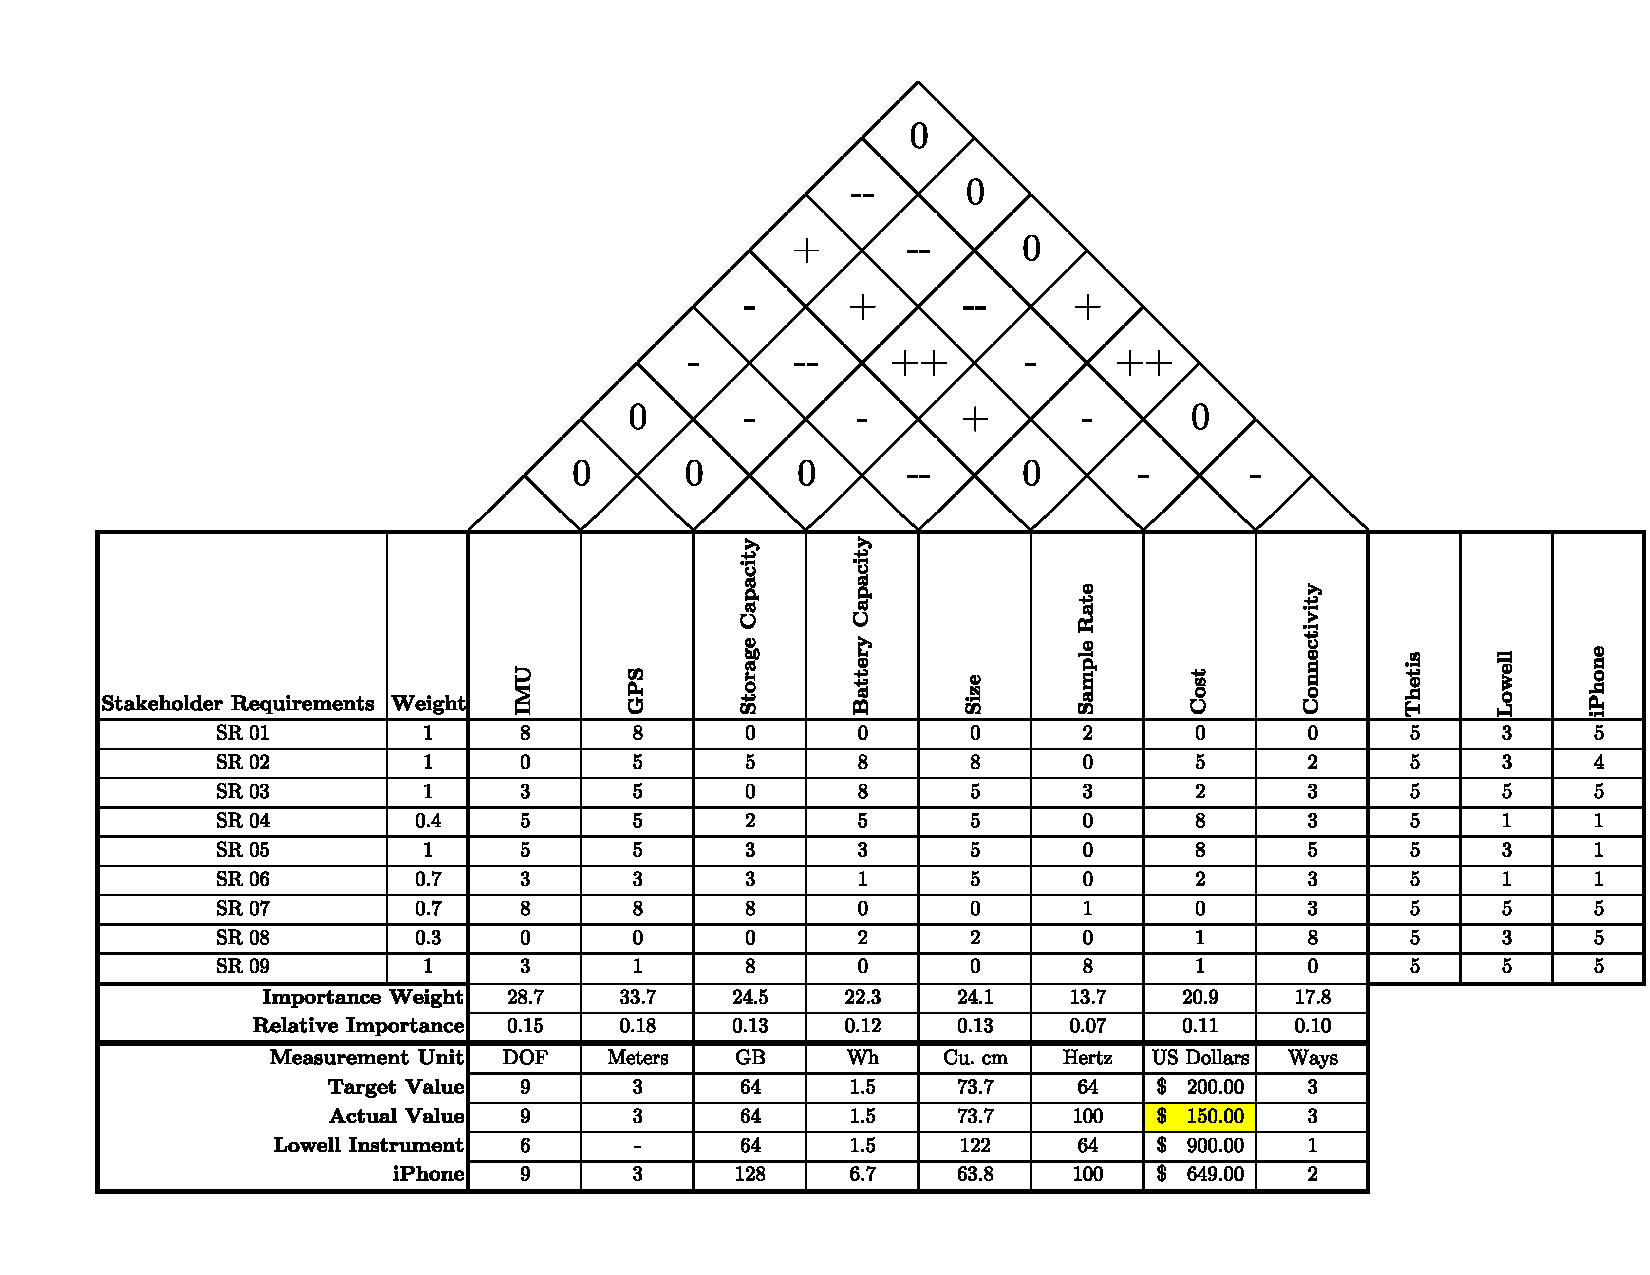
\includepdf[landscape=true]{C:/Users/bduffy2018/OneDrive - Florida Institute of Technology/School/Thesis/Design Dossier/ThetisHOQ.pdf}
\end{landscape}

\section{Concept of Operations} \label{sec:conops}

\section{Conceptual Design} \label{sec:conceptual_design}

\subsection{Functional Block Diagram} \label{ssec:block_diagram}

\subsection{Functional Flow Diagram} \label{ssec:flow_diagram}

\subsection{Available Commercial Off the Shelf Products} \label{ssec:cots_products}

\subsection{Analytical Hierarchy Process} \label{ssec:ahp}

\subsubsection*{Inertial Measurement Unit} \label{sssec:ahp_imu}

\subsection{Failure Mode, Effect, and Criticality Analysis} \label{ssec:fmeca}